\chapter{Resultados} \label{chap:resultados}

Neste capítulo, os resultados obtidos neste trabalho são abordados com o intuito de explicá-los ao leitor e de realizar uma breve análise englobando as expectativas iniciais do autor e possíveis consequências dos resultados obtidos.

\section{Avaliação de modelos de treinamento}

Esta seção tem como objetivos descrever brevemente as avaliações realizadas, identificar os melhores modelos de treinamento dentre os modelos avaliados e analisar os resultados obtidos pelos melhores modelos de treinamento. Acreditamos que, dessa forma, o leitor será primeiro provido das informações relevantes das avaliações realizadas para apenas então ser apresentado aos resultados e análises baseados nessas avaliações.

\subsection{Descrição das avaliações realizadas}

No total, foram realizadas 30 avaliações de modelos de treinamento de aprendizado de máquina, 18 para modelos do tipo perceptron multicamada e 12 para modelos do tipo floresta aleatória. Estas avaliações permitiram que um total de 5346 modelos de treinamento fossem avaliados segundo o método de avaliação proposto, sendo 90 destes modelos do tipo perceptron multicamada e 5256 destes modelos do tipo floresta aleatória. Por fim, podemos observar que, dentre os modelos testados, um total de 18 modelos do tipo perceptron multicamada e 1053 modelos do tipo floresta aleatória foram classificados entre os melhores 20\% de todos os modelos de sua avaliação no quesito melhor média de acurácia para os dados de validação e, assim, foram testados em todos os 100 subconjuntos de teste disponíveis.

Podemos observar na Tabela \ref{table:descricao_avaliacoes_perceptron_multicamada} uma breve descrição de cada avaliação realizada para modelos do tipo perceptron multicamada e na Tabela \ref{table:descricao_avaliacoes_floresta_randomica} uma descrição análoga de cada avaliação realizada para modelos do tipo floresta aleatória. Estas descrições abordam os números das avaliações, o número de modelos avaliados, e as variações de hiperparâmetros empregadas. Para conveniência do leitor e concisão deste texto, as descrições de avaliações feitas para diferentes tipos de modelos de treinamento foram separadas em diferentes tabelas e algumas avaliações foram agrupadas na mesma descrição devido à sua semelhança nas variações de hiperparâmetros. As avaliações realizadas foram estruturadas de modo a testar uma grande quantidade de variações de hiperparâmetros para cada tipo de modelo com o intuito de determinar o conjunto de hiperparâmetros mais apto para uso em uma aplicação prática no website auxiliar. Em certos casos, os resultados de uma avaliação influenciaram diretamente as variações de hiperparâmetros das avaliações subsequentes.

\begin{table}[ht!]
  \begin{center}
  \setlength{\belowcaptionskip}{10pt}
  \footnotesize {
    \begin{tabular}{|p{1.5cm}|p{2cm}|p{12cm}|}
	  \hline
	  \textbf{Avalições} & \textbf{Número total de modelos} & \textbf{Variações de hiperparâmetros} \\
	  \hline
    03 & 5 & Perceptron multicamada com 1 camada de entrada, 1 camada escondida e 1 camada de saída. Variação do tamanho da camada escondida no intervalo $[100 .. 500]$ com deslocamentos de 100 em 100. Máximo de épocas de treinamento: 15 mil.\\
    \hline
    04, 05, 08, 09, 10 & 25 & Perceptron multicamada com 1 camada de entrada, 2 camadas escondidas e 1 camada de saída. Variação do tamanho da primeira camada escondida no intervalo $[100 .. 500]$ com deslocamentos de 100 em 100 e do tamanho da segunda camada escondida no intervalo $[20 .. 100]$ com deslocamentos de 20 em 20. Máximo de épocas de treinamento: 15 mil. \\
    \hline
    19 & 5 & Perceptron multicamada com 1 camada de entrada, 1 camada escondida, 1 camada com \textit{dropout} com taxa de 0.2 e 1 camada de saída. Variação do tamanho da camada escondida no intervalo $[100 .. 500]$ com deslocamentos de 100 em 100. Máximo de épocas de treinamento: 20 mil. \\
    \hline
    20 - 24 & 25 & Perceptron multicamada com 1 camada de entrada, 2 camadas escondidas, 2 camadas com \textit{dropout} com taxa de 0.2 (intercaladas na sequência camada escondida seguida de camada com \textit{dropout}) e 1 camada de saída. Variação do tamanho da primeira camada escondida no intervalo $[100 .. 500]$ com deslocamentos de 100 em 100 e do tamanho da segunda camada escondida no intervalo $[20 .. 100]$ com deslocamentos de 20 em 20. Máximo de épocas de treinamento: 20 mil. \\
    \hline
    25 & 5 & Perceptron multicamada com 1 camada de entrada, 1 camada escondida com regularização de \textit{kernel} L2 com taxa 0.01 e 1 camada de saída. Variação do tamanho da camada escondida no intervalo $[100 .. 500]$ com deslocamentos de 100 em 100. Máximo de épocas de treinamento: 20 mil. \\
    \hline
    26 - 30 & 25 & Perceptron multicamada com 1 camada de entrada, 2 camadas escondidas com regularização de \textit{kernel} L2 com taxa 0.01 e 1 camada de saída. Variação do tamanho da primeira camada escondida no intervalo $[100 .. 500]$ com deslocamentos de 100 em 100 e do tamanho da segunda camada escondida no intervalo $[20 .. 100]$ com deslocamentos de 20 em 20. Máximo de épocas de treinamento: 20 mil. \\
    \hline
    \end{tabular}
  }
  \caption{Breve descrição das avaliações realizadas para modelos de treinamento do tipo perceptron multicamada.}
  \label{table:descricao_avaliacoes_perceptron_multicamada}
  \end{center}
\end{table}

\begin{table}[ht!]
  \begin{center}
  \setlength{\belowcaptionskip}{10pt}
  \footnotesize {
    \begin{tabular}{|p{1.5cm}|p{2cm}|p{12cm}|}
	  \hline
	  \textbf{Avalições} & \textbf{Número total de modelos} & \textbf{Variações de hiperparâmetros} \\
	  \hline
	  01 & 30 & Variação do número de estimadores no intervalo $[10 .. 300]$ com deslocamentos de 10 em 10. Critério de divisão gini. Raiz quadrada do total de características como número máximo de características analisadas em uma divisão. \\
	  \hline
    02 & 60 & Variação do número de estimadores no intervalo $[190 .. 230]$ com deslocamentos de 5 em 5. Critérios de divisão: gini e entropia. Número máximo de características analisadas em uma divisão: raiz quadrada do total de características, logaritmo de base 2 do total de características e ausência de número máximo de características analisadas. \\
    \hline
    06 & 90 & 210 estimadores. Critério de divisão gini. Raiz quadrada do total de características como número máximo de características analisadas em uma divisão. Variação do mínimo de amostras para gerar uma folha no intervalo $[1 .. 10]$ e do mínimo de amostras para dividir um nó interno no intervalo $[2 .. 10]$. \\
    \hline
    07 & 450 & Variação do número de estimadores no intervalo $[200 .. 220]$ com deslocamentos de 5 em 5. Critérios de divisão: gini e entropia. Número máximo de características analisadas em uma divisão: raiz quadrada do total de características, logaritmo de base 2 do total de características e ausência de número máximo de características analisadas. Variação do mínimo de amostras para gerar uma folha no intervalo $[1 .. 3]$ e do mínimo de amostras para dividir um nó interno no intervalo $[5 .. 9]$. \\
    \hline
    11 & 66 & 210 estimadores. Critérios de divisão: gini e entropia. Número máximo de características analisadas em uma divisão: raiz quadrada do total de características, logaritmo de base 2 do total de características e ausência de número máximo de características analisadas. Variação da profundidade máxima das árvores no intervalo $[2 .. 12]$. \\
    \hline
    12, 13, 14 & 2250 & Variação do número de estimadores no intervalo $[200 .. 220]$ com deslocamentos de 5 em 5. Critérios de divisão: gini e entropia. Número máximo de características analisadas em uma divisão: raiz quadrada do total de características, logaritmo de base 2 do total de características e ausência de número máximo de características analisadas. Variação do mínimo de amostras para gerar uma folha no intervalo $[1 .. 3]$; do mínimo de amostras para dividir um nó interno no intervalo $[5 .. 9]$; e da profundidade máxima das árvores no intervalo $[2 .. 6]$. \\
    \hline
    15 & 66 & 210 estimadores. Critérios de divisão: gini e entropia. Número máximo de características analisadas em uma divisão: raiz quadrada do total de características, logaritmo de base 2 do total de características e ausência de número máximo de características analisadas. Variação do número máximo de folhas das árvores no intervalo $[4 .. 24]$ com deslocamentos de 2 em 2. \\
    \hline
    16, 17, 18 & 2250 & Variação do número de estimadores no intervalo $[200 .. 220]$ com deslocamentos de 5 em 5. Critérios de divisão: gini e entropia. Número máximo de características analisadas em uma divisão: raiz quadrada do total de características, logaritmo de base 2 do total de características e ausência de número máximo de características analisadas. Variação do mínimo de amostras para gerar uma folha no intervalo $[1 .. 3]$; do mínimo de amostras para dividir um nó interno no intervalo $[5 .. 9]$; e do número máximo de folhas das árvores no intervalo $[16 .. 20]$.  \\
    \hline
    \end{tabular}
  }
  \caption{Breve descrição das avaliações realizadas para modelos de treinamento do tipo floresta aleatória.}
  \label{table:descricao_avaliacoes_floresta_randomica}
  \end{center}
\end{table}

Como já explicado no capítulo \ref{chap:procedimento_adotado}, a discrepância entre o número de modelos por avaliação e o número de avaliações em si para os modelos do tipo floresta aleatória e do tipo perceptron multicamada ocorre pois as avaliações feitas pelo autor com modelos do tipo perceptron multicamada foram consideravelmente lentas.

\subsection{Melhores resultados}

Dentre os 18 modelos do tipo perceptron multicamada e 1053 modelos do tipo floresta aleatória testados nos 100 subconjuntos de teste disponíveis, podemos observar os resultados dos 3 melhores modelos do tipo perceptron multicamada e dos 5 melhores modelos do tipo floresta aleatória na Tabela \ref{table:ranking_melhores_modelos}, na qual os modelos foram rankeados pelo critério de melhor média de acurácia para os dados de teste.

\begin{table}[ht!]
  \begin{center}
  \setlength{\belowcaptionskip}{10pt}
  \footnotesize {
    \begin{tabular}{|p{1.25cm}|p{2cm}|p{2cm}|p{2.5cm}|p{6.75cm}|}
	  \hline
	  \textbf{Ranking} & \textbf{Tipo de \newline modelo} & \textbf{Identificação do modelo} & \textbf{Médias de \newline acurácia} & \textbf{Descrição do modelo} \\
	  \hline
    1º & Floresta \newline aleatória & Número da \newline avaliação: 18 \newline Número do \newline modelo: 21 & Teste: 0.760 \newline Validação: 0.762 & 215 estimadores. Critério de divisão gini. Ausência de número máximo de características analisadas em uma divisão. Mínimo de 3 amostras para gerar uma folha. Mínimo de 8 amostras para dividir um nó interno. Máximo de 19 folhas por árvore. \\
    \hline
    2º & Floresta \newline aleatória & Número da \newline avaliação: 18 \newline Número do \newline modelo: 58 & Teste: 0.760 \newline Validação: 0.759 & 220 estimadores. Critério de divisão gini. Ausência de número máximo de características analisadas em uma divisão. Mínimo de 2 amostras para gerar uma folha. Mínimo de 8 amostras para dividir um nó interno. Máximo de 19 folhas por árvore. \\
    \hline
    3º & Floresta \newline aleatória & Número da \newline avaliação: 18 \newline Número do \newline modelo: 25 & Teste: 0.759 \newline Validação: 0.761 & 210 estimadores. Critério de divisão gini. Ausência de número máximo de características analisadas em uma divisão. Mínimo de 3 amostras para gerar uma folha. Mínimo de 9 amostras para dividir um nó interno. Máximo de 20 folhas por árvore. \\
    \hline
    4º & Floresta \newline aleatória & Número da \newline avaliação: 18 \newline Número do \newline modelo: 27 & Teste: 0.759 \newline Validação: 0.761 & 205 estimadores. Critério de divisão gini. Ausência de número máximo de características analisadas em uma divisão. Mínimo de 3 amostras para gerar uma folha. Mínimo de 9 amostras para dividir um nó interno. Máximo de 20 folhas por árvore. \\
    \hline
    5º & Floresta \newline aleatória & Número da \newline avaliação: 18 \newline Número do \newline modelo: 49 & Teste: 0.759 \newline Validação: 0.760 & 200 estimadores. Critério de divisão gini. Ausência de número máximo de características analisadas em uma divisão. Mínimo de 3 amostras para gerar uma folha. Mínimo de 9 amostras para dividir um nó interno. Máximo de 17 folhas por árvore. \\
    \hline
    6º & Perceptron multicamada & Número da \newline avaliação: 09 \newline Número do \newline modelo: 00 & Teste: 0.707 \newline Validação: 0.694 & 1 camada de entrada, 1 camada escondida de 400 unidades, 1 camada escondida de 20 unidades e 1 camada de saída. Máximo de épocas de treinamento: 15 mil. \\
    \hline
    7º & Perceptron multicamada & Número da \newline avaliação: 24 \newline Número do \newline modelo: 00 & Teste: 0.704 \newline Validação: 0.716 & 1 camada de entrada, 1 camada escondida de 500 unidades, 1 camada com \textit{dropout} com taxa de 0.2, 1 camada escondida de 100 unidades, 1 camada com \textit{dropout} com taxa de 0.2 e 1 camada de saída. Máximo de épocas de treinamento: 20 mil. \\
    \hline
    8º & Perceptron multicamada & Número da \newline avaliação: 30 \newline Número do \newline modelo: 00 & Teste: 0.700 \newline Validação: 0.704 & 1 camada de entrada, 1 camada escondida de 500 unidades com regularização de \textit{kernel} L2 com taxa 0.01, 1 camada escondida de 100 unidades com regularização de \textit{kernel} L2 com taxa 0.01 e 1 camada de saída. Máximo de épocas de treinamento: 20 mil. \\
    \hline
    \end{tabular}
  }
  \caption{Ranking dos 3 melhores modelos do tipo perceptron multicamada e dos 5 melhores modelos do tipo floresta aleatória segundo a média de acurácia para dados de teste.}
  \label{table:ranking_melhores_modelos}
  \end{center}
\end{table}

Para permitir ao leitor analisar com maior profundidade os resultados obtidos pelo modelo de treinamento que será utilizado para a previsão de dados no website, os gráficos de resultados para os subconjuntos de validação e teste do melhor modelo do rankeamento apresentado na Tabela \ref{table:ranking_melhores_modelos} foram disponibilizados na imagem \ref{fig:best_results_plot}.

\begin{figure}[h]
	\centering
  \subfigure[Gráfico de barras]{
    \centering
    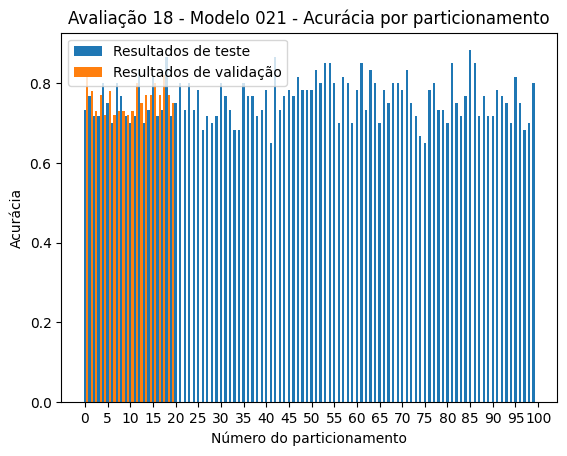
\includegraphics[scale=0.5]{images/grafico_barras_resultados_melhor_modelo.png}
    \label{fig:best_results_barplot}
  }
  \subfigure[Gráfico de caixa]{
    \centering
    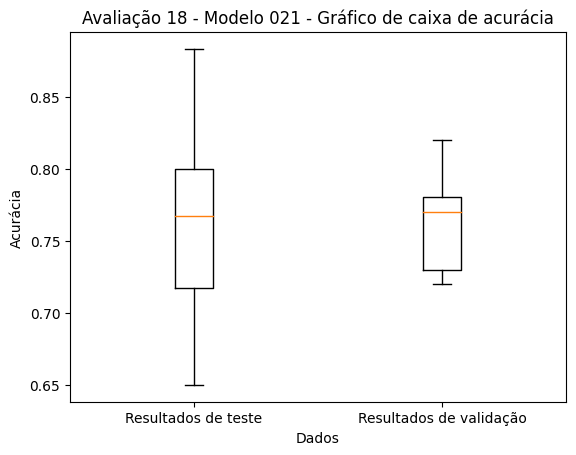
\includegraphics[scale=0.5]{images/grafico_caixa_resultados_melhor_modelo.png}
    \label{fig:best_results_boxplot}
  }
  \subfigure[Histograma]{
    \centering
    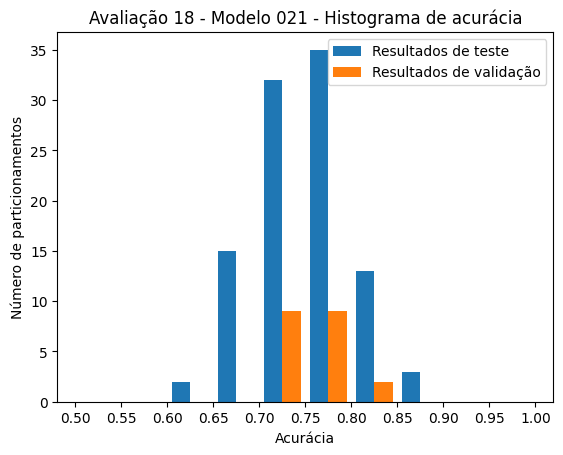
\includegraphics[scale=0.5]{images/histograma_resultados_melhor_modelo.png}
    \label{fig:best_results_histogram}
  }
	\caption{Gráficos de resultados para o melhor modelo do rankeamento.}
	\label{fig:best_results_plot}
\end{figure}

Com as informações apresentadas na Tabela \ref{table:ranking_melhores_modelos}, poderemos realizar uma análise entre os diferentes tipos de modelos de treinamento e em relação à escolha de hiperparâmetros de cada tipo de modelo de treinamento. Também poderemos comparar os resultados obtidos neste trabalho com os resultados obtidos no artigo de Chicco e Jurman \cite{chicco2020}, o qual utilizou o mesmo conjunto de dados \cite{larxel_dataset} para avaliação de modelos de aprendizado de máquina.

Como observado na Tabela \ref{table:ranking_melhores_modelos}, podemos notar que os 5 melhores modelos de florestas aleatórias tiveram um desempenho superior em relação aos 3 melhores modelos do tipo perceptron multicamada. Embora isso possa ter sido exacerbado pela discrepância entre o número de modelos avaliados do tipo floresta aleatória e do tipo perceptron multicamada, esse resultado já era esperado antes da realização das avaliações. Isso porque o artigo de Chicco e Jurman também havia verificado um melhor desempenho dos modelos de treinamento do tipo floresta aleatória em relação aos modelos de treinamento do tipo perceptron multicamada no conjunto de dados utilizado, corroborando os resultados obtidos neste trabalho.

Analisando os hiperparâmetros dos modelos do tipo floresta aleatória, podemos realizar algumas constatações. Primeiramente, podemos notar que o número de estimadores utilizados não parece ter sido uma característica que influenciou significativamente os resultados, pois todos os 5 valores de número de estimadores utilizados na avaliação 18 produziram um modelo no ranking de melhores modelos. Além disso, podemos também constatar que a utilização do coeficiente de gini se mostrou superior ao uso da entropia como critério de divisão. Também observamos que a ausência de um número máximo de características consideradas por divisão superou o uso de um número máximo de características consideradas por divisão sendo igual à raiz quadrada do total de características ou ao logaritmo de base 2 do total de características, o que contraria a teoria existente segundo a qual o uso da raiz quadrada do total de características como número máximo de características consideradas por divisão forneceria os melhores resultados \cite[p.319-321]{statistical_learning}. Outro aspecto que podemos observar é que a utilização de técnicas para limitar o número de divisões das árvores (mínimo de amostras para gerar uma folha, mínimo de amostras para dividir um nó interno) se mostraram úteis na obtenção dos melhores resultados, pois todos eles fizeram uso de ambas. Por fim, notamos que tanto a limitação no número de folhas como a limitação da profundidade máxima das árvores produziram bons resultados (embora esta última não tenha sido utilizada por nenhum dos melhores resultados, seu uso levou a um aumento da acurácia em relação a árvores que não a utilizaram). As duas últimas observações estão de acordo com a teoria por trás do modelo de árvores de decisão segundo a qual árvores complexas levam a \textit{overfitting} dos dados de treino, de forma que recursos para limitar a complexidade de uma árvore ou para extrair uma sub-árvore da árvore final podem diminuir o erro obtido sobre o subconjunto de dados de teste \cite[p.307-311]{statistical_learning}.

Analisando os hiperparâmetros dos modelos do tipo perceptron multicamada, também podemos realizar algumas constatações. Em primeiro lugar, notamos que todos os modelos de perceptrons multicamada presentes no ranking apresentam duas camadas escondidas, indicando que os modelos com duas camadas escondidas obtiveram melhor desempenho do que os modelos com apenas uma camada escondida. Também é possível observar que os modelos com maior número de unidades nas camadas escondidas forneceram um melhor desempenho, em especial se combinados com um maior número de épocas de treinamento e uma camada com \textit{dropout} ou um \textit{kernel} de regularização aplicado aos pesos das camadas escondidas, tendo-se em vista que os 2 últimos modelos do tipo perceptron multicamada presentes no ranking possuem a maior quantidade de unidades para ambas as camadas escondidas dentre todos os modelos avaliados. O fato de o melhor modelo do tipo perceptron multicamada ter sido um modelo com camadas escondidas de tamanho 400 e 20, que não utiliza \textit{dropout} ou um \textit{kernel} de regularização aplicado aos pesos das camadas escondidas e que teve um limite máximo de 15 mil épocas de treinamento é um pouco surpreendente, em especial se considerarmos a média de acurácia para os dados de validação obtida por esse modelo. Com os resultados obtidos até aqui, creio que essa última constatação não possa ser explicada de maneira satisfatória, sendo necessária a realização de mais avaliações para se chegar a um resultado conclusivo.

Comparando os resultados obtidos neste trabalho com os resultados obtidos sobre o mesmo conjunto de dados no artigo de Chicco e Jurman, podemos constatar que as avaliações realizadas neste trabalho obtiveram um bom desempenho. No artigo de Chicco e Jurman, cujo método de avaliação utilizado está descrito no capítulo \ref{chap:procedimento_adotado}, os melhores resultados de acurácia de previsão para o subconjunto de teste foram de 0.740 e de 0.680, respectivamente, para modelos do tipo floresta aleatória e perceptron multicamada. Em comparação, os melhores resultados de acurácia de previsão para o subconjunto de teste obtidos neste trabalho e apresentados na Tabela \ref{table:ranking_melhores_modelos} foram de 0.760 e 0.707, respectivamente, para modelos do tipo floresta aleatória e perceptron multicamada. Como os métodos de avaliação utilizados neste trabalho e no artigo de Chicco e Jurman diferem em alguns aspectos, não podemos afirmar conclusivamente que este trabalho conseguiu melhorar os resultados existentes para esse conjunto de dados, mas podemos afirmar que os resultados obtidos neste trabalho se encaixam nas expectativas estabelecidas pelo artigo de Chicco e Jurman.

\section{Website}

O resultado a ser apresentado relativo ao website seria o website em si, o qual funcionou adequadamente, permitindo que um usuário criasse pacientes e requisitasse previsões de sobrevivência à insuficiência cardíaca para estes, as quais foram processadas pelo \textit{backend} e tiveram seus resultados fornecidos. Porém, como não é possível apresentar todo o website e seu funcionamento neste documento, algumas páginas do website foram fornecidas com o intuito de ilustar a aplicação desenvolvida.

Na imagem \ref{fig:website_login_page} temos a página de login, que descreve o website ao usuário e permite que este realize login no website ou seja direcionado para a página de cadastro. Na imagem \ref{fig:website_home_page} temos a página principal do usuário, na qual os pacientes deste podem ser visualizados e gerenciados. Por fim, na imagem \ref{fig:website_patient_predictions_page} temos a página de previsões de um paciente, onde podemos visualizar as informações de um paciente e suas previsões realizadas e excluir previsões indesejadas.

\begin{figure}[ht!]
	\centering
  
\includegraphics[scale=0.26]{images/website_pagina_login.png}
  \caption{Página de login do website}
  \label{fig:website_login_page}
\end{figure}

\begin{figure}[ht!]
  \centering
  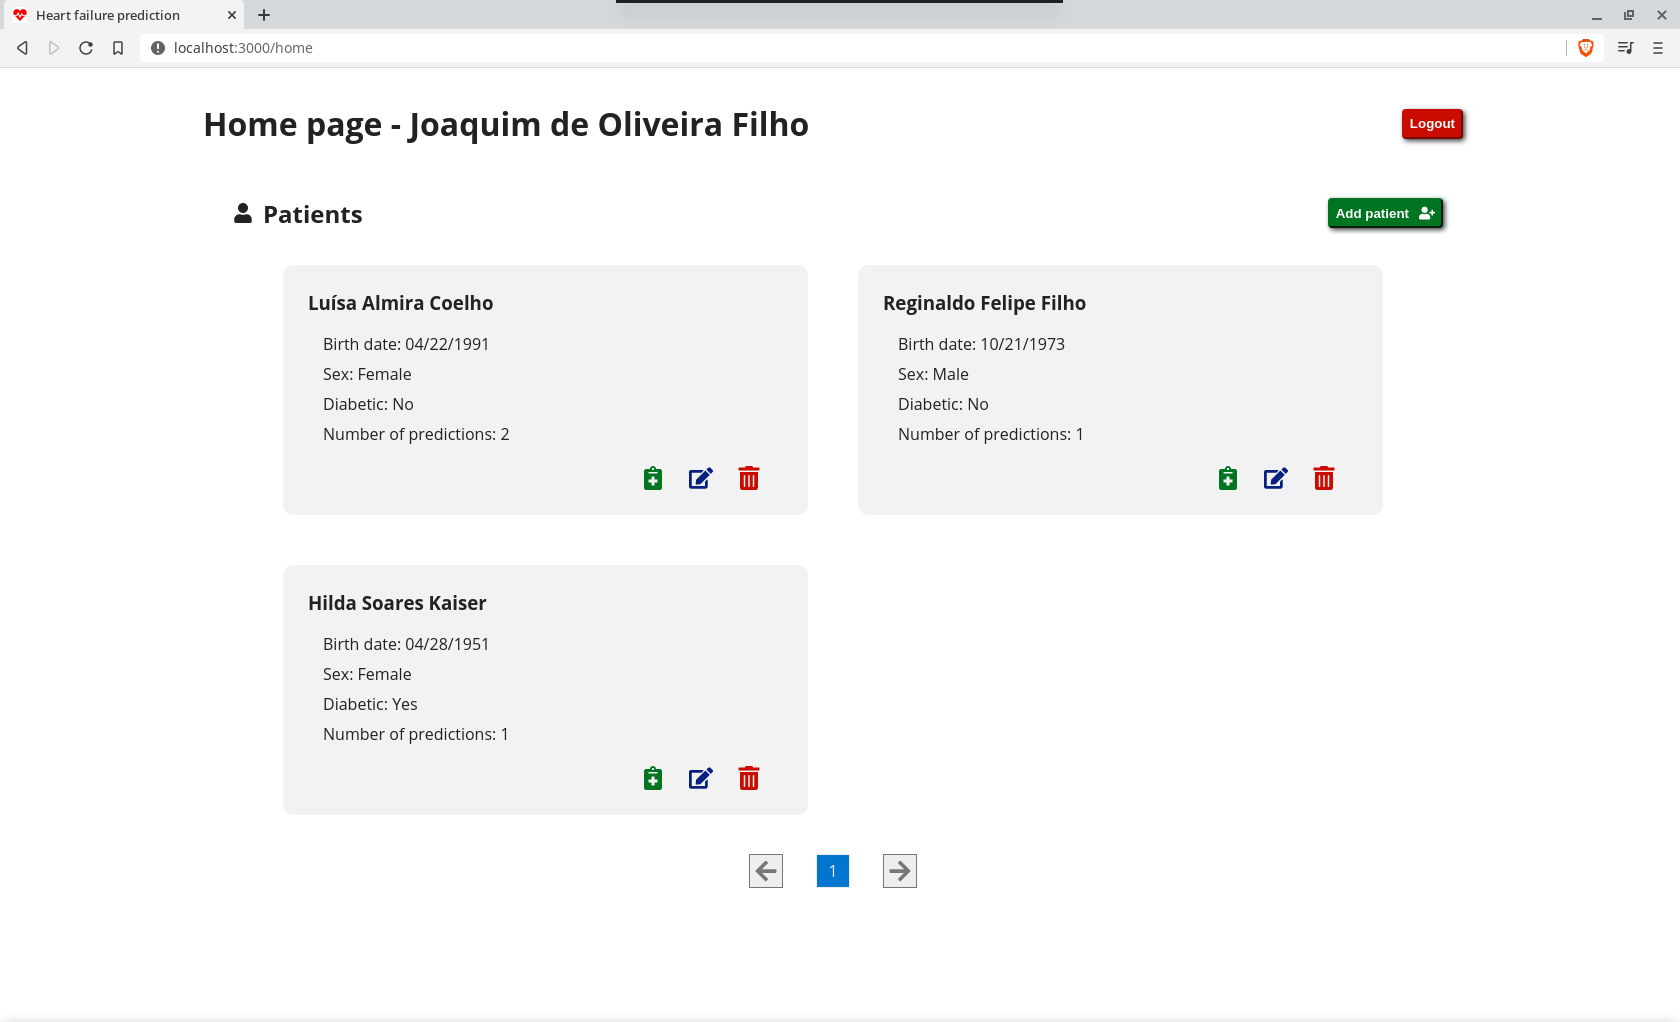
\includegraphics[scale=0.26]{images/website_pagina_home.png}
  \caption{Página principal do usuário do website}
  \label{fig:website_home_page}
\end{figure}

\begin{figure}[ht!]
  \centering
  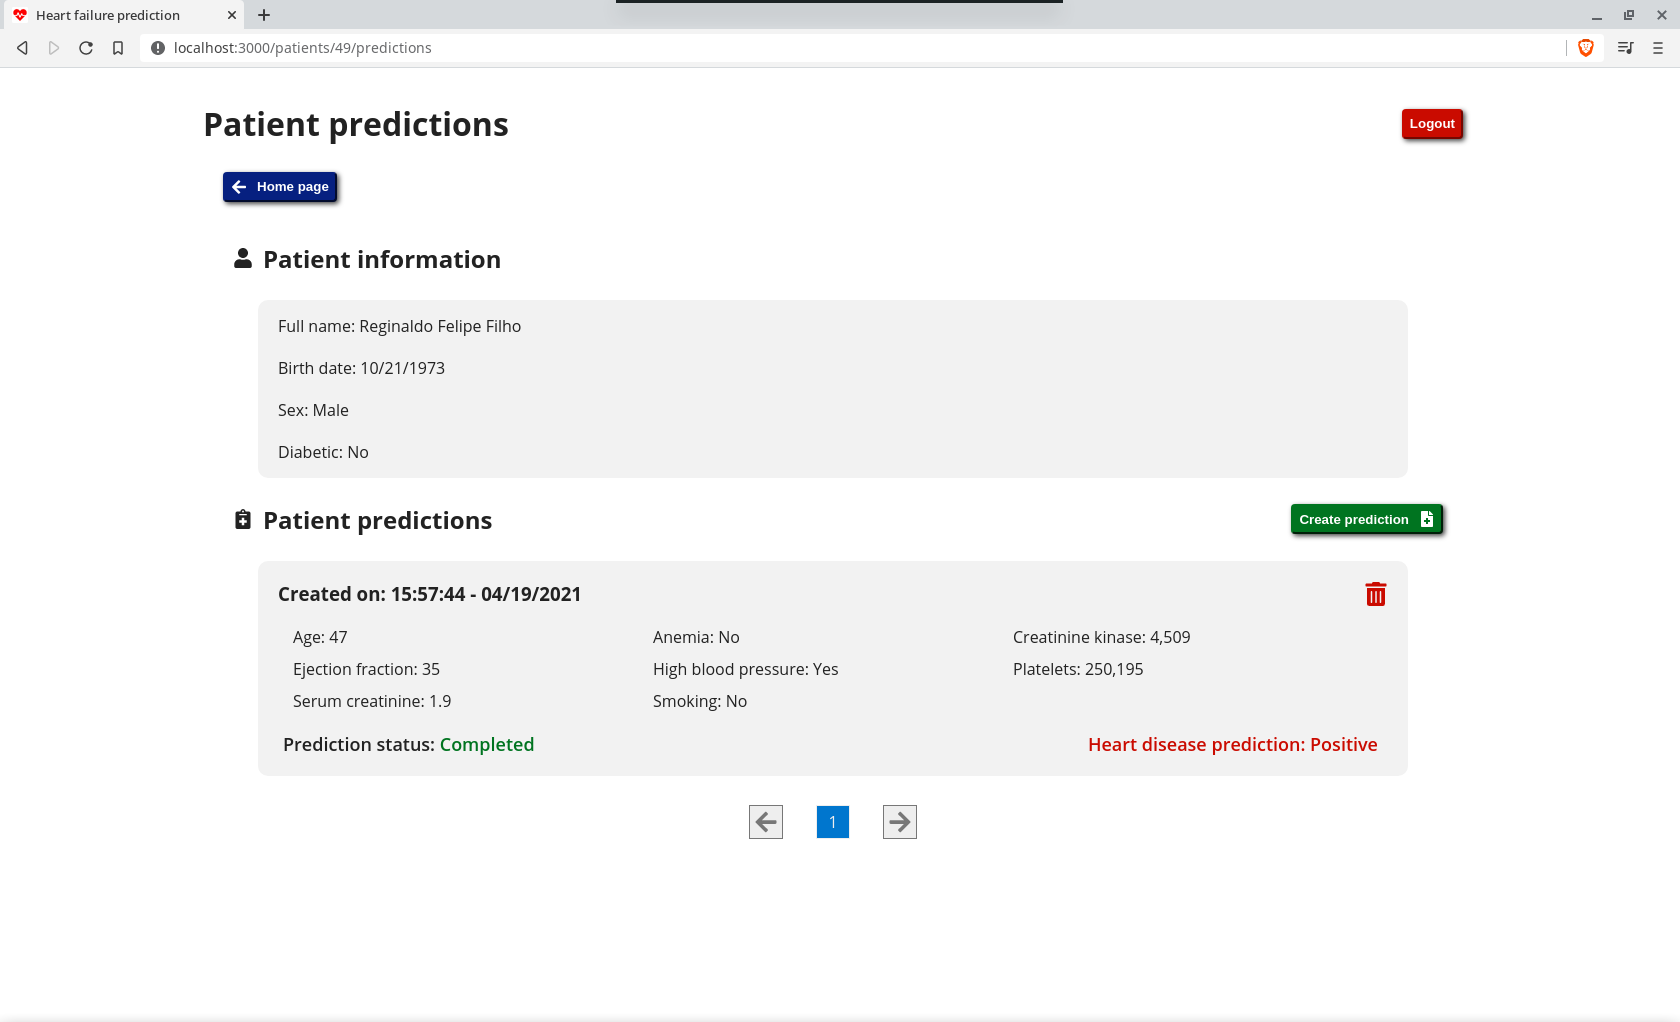
\includegraphics[scale=0.26]{images/website_pagina_previsoes_paciente.png}
  \caption{Página de previsões de um paciente do website}
  \label{fig:website_patient_predictions_page}
\end{figure}

Caso o leitor deseje explorar o funcionamento do website mais a fundo ou entender detalhes de sua implementação, o código fonte tanto do \textit{backend} como do \textit{frontend} pode ser encontrado no repositório do \textit{GitHub} deste trabalho\footnote{\url{https://github.com/AndreLaranjeira/ML-HeartFailureSurvival}}.

No próximo capítulo, apresentaremos as conclusões que resultaram deste trabalho e propostas para trabalhos futuros.
